\documentclass[11pt]{article}
\usepackage{fullpage}
\usepackage{setspace}
\usepackage{amsmath}
\usepackage{fancyvrb}
\usepackage{enumerate}
\usepackage{listings}
\usepackage{pgfplots}
\usepackage{graphicx}
\usepackage{float}
\usepackage{multirow}
\usepackage[format=hang,labelsep=quad]{caption}
\usepackage{subfig}
\usepackage{array}
\usepackage{multirow}
\usepackage[final]{pdfpages}

\renewcommand\thesubfigure{\roman{subfigure}}


\begin{document}
\noindent\large{Math 5364}\\
\large{Data Mining 2}\\
\large{Homework 31}\\
\large{Mary Barker}

\begin{enumerate}
\item The file Hw31data.txt contains SAS code for generating two data sets. 
	The first data set provides the correlation matrix of six measurement 
	made on white leghorn fowls, including skull length(SL), skull 
	breadth (SB), humerus length (HS), ulna length (UL), femur length 
	(FL), and tibia length(TL);

\begin{Verbatim}
	%include '/folders/myshortcuts/sas_folder/Hw31Data.txt';
\end{Verbatim}

	\begin{enumerate}
	\item 
	Perform a principal components analysis for this data set, and 
		report the resulting eigenvalues and eigenvectors;

\begin{Verbatim}
		proc princomp data = leghorn;
		run;
\end{Verbatim}
		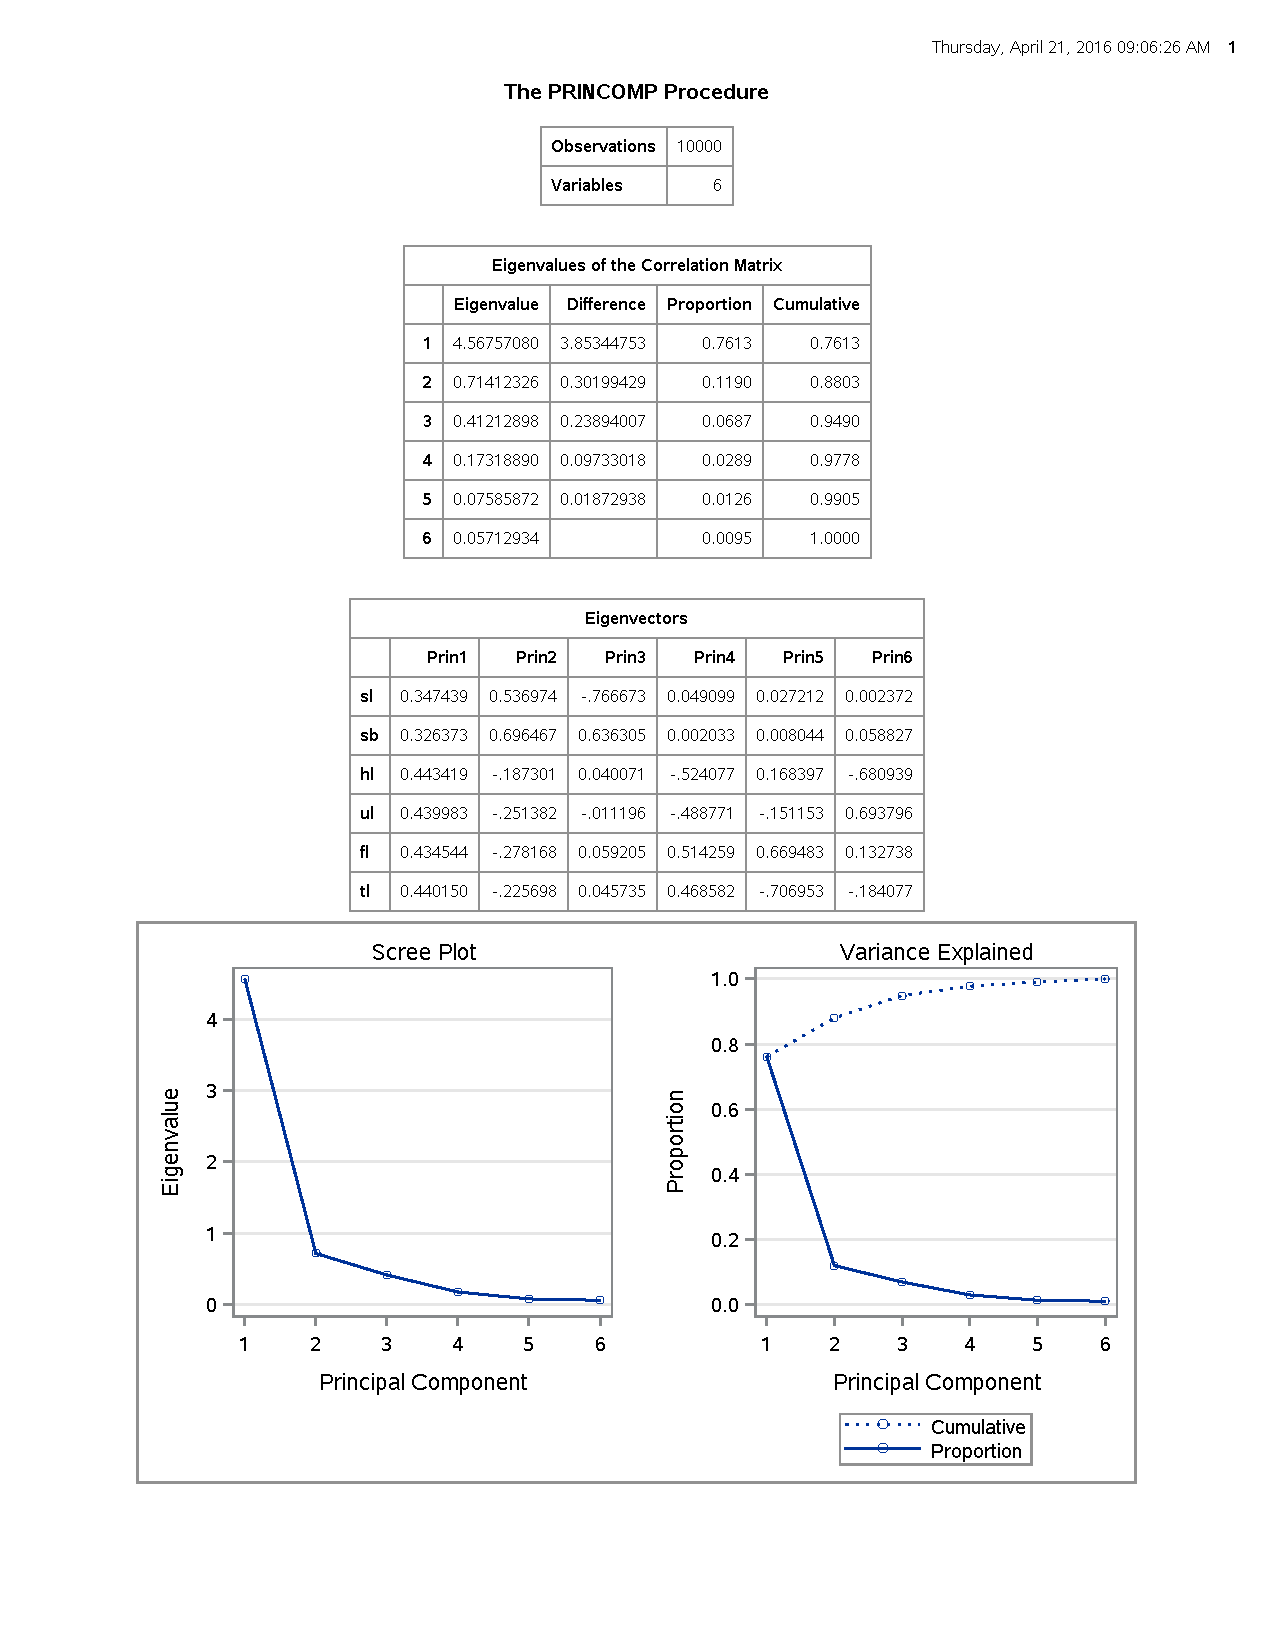
\includepdf[pages={1}]{hw31-results.pdf}

	\item 
	How many principal components are required to explain at least 
		90\% of the total variation in the data? ;

		3

	\item 
	Provide an intuitive interpretation for the principal components 
		accounting for 90\% of the total variation. (For example, the 
		first principal component has large positive coefficients for 
		all of the variables in the data set, so it roughly measure 
		the overall size of a white leghorn fowl.);

			The first principal component has relatively uniform values 
			for coefficients, giving overall an indication of how big each animal is. 

			The second principal component has large coefficients for 
			SB and SL, and negative, not to say small coefficients 
			for the other variables, indicating a description of 
			just how big the skull is.

			The third component has larger absolute values for SB and SL, 
			as with the second, but the value for SL is negative, so 
			this seems to evaluate the difference between skull width 
			and height.
	\end{enumerate}

\item  Perform a factor analysis on the leghorn data;

\begin{Verbatim}
	proc factor data=leghorn res;
	run;
\end{Verbatim}

	\begin{enumerate}
	\item 
	How many factors are retained using the MINEIGEN criterion?
\begin{Verbatim}
		proc factor data=leghorn mineigen=0.05;
		run;
\end{Verbatim}
		Only one factor was retained. 
		\includepdf[pages={3-4}]{hw31-results.pdf}

	\item 
	What is the overall RMS off-diagonal residuals in this case?

	0.08123310

	\end{enumerate}

\item Continuing with the leghorn data set, increase the number of factors 
	until the overall residual RMS is less than 0.05;

\begin{Verbatim}
	proc factor data=leghorn nfact=3 res;
	run;
\end{Verbatim}
	\includepdf[pages={8-9}]{hw31-results.pdf}

	\begin{enumerate}
	\item How many factors are required to achieve this?

		3 factors

	\item Report the estimated matrices hatL and hat Phi

		

	\item What is the communality for skull length?

		$\approx$ 0.9995. 

	\item Find the unique variance of ulna length

		0.07061

	\item What is the correlation between femur length and the 2nd factor?

	\end{enumerate}

\item The second data set in Hw31data.txt contains responses of 122 
	diabetes patients to 25 survey questions, on a Likert scale 
	(a scale typically used on surveys, where 
		1 = Strongly Disagree, 
		2 = Somewhat Disagree, 
		3 = Neither DIsagree Nor Agree, 
		4 = Somewhat Agree, and 
		5 = Strongly Agree
	). 

	\begin{enumerate}
	\item Perform a factor analysis with nfact=17 on this data and store 
		the factor scores in a data set.

\begin{Verbatim}
	proc factor data=diabetes score nfact=17 res out = fact_scores;
	run;
\end{Verbatim}
	\includepdf[pages={11-13}]{hw31-results.pdf}

	\item One of the assumptions of the factor model is that 
		cov(f) = identity. Verify that the sample covariance matrix of 
		the factor scores is equal to I (This occurs exactly, because 
		we are using the principal component method for this factor 
		analysis. There are other methods where this does not occur.)

\begin{Verbatim}
	proc corr data=fact_scores cov;
		var Factor1-Factor17;
	run;
\end{Verbatim}
	\includepdf[pages={25}]{hw31-results.pdf}

	\item What does cov($f$) = $I$ say about the correlation between the two 
		different factors? What would you expect the scatter plot of 
		the two different factors to look like?

		That the covariance matrix is $I$ measn that the factors are 
		uncorrelated, or independent. 
		I would expect the plot to look random, with no underlying pattern between 
		the two variables. 
		

	\item Create a scatter plot of f1 vs f2. Does this plot agree with 
		your expectations? ;

\begin{Verbatim}
	proc plot data=fact_scores;
		plot Factor1*Factor2;
	run;
\end{Verbatim}

	\includepdf[pages={30}]{hw31-results.pdf}
	My initial guess does seem to be supported by the graph, where there 
	is no trend discernible. 

	\item It would be interesting to interpret the factors in this 
		problem, but in order to do that, we will need to consider 
		rotations of the factors, so this will have to wait until a 
		future homework assignment. 

	\end{enumerate}
\end{enumerate}
\end{document}
